\documentclass[journal abbreviation, manuscript]{copernicus}

\begin{document}

 %% \ SECTION 3
\section{Use cases}
Andrew Comments:

Structure: just go through it, Use Case I, Use Case II, Use Case II. No Methods & Results section

go through it from front to back, explain what an NPZD model is.
"We recreate the NPZD model formulation by Anderson, in the model there is one .." describe equations in words. Then say See Anderson et al. or appendix X for full equations



- jupyter notebook for each example

\subsection{Methods}
%  quickly explain overview, explain methods for all of them shortly, with schematics, and put full system of equations & parameter tables in the Appendix!
\subsubsection{Forcing}
%%f
\begin{figure*}[t]
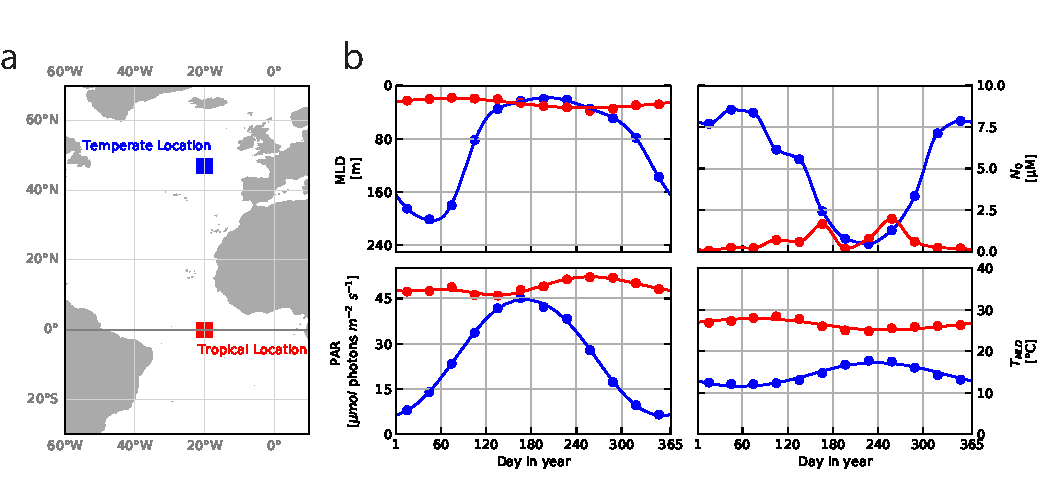
\includegraphics[width=15cm]{Figures/firstdraft_plots/01_forcing_labeled.pdf}
\caption{(a) Map shows locations of the two comparative model runs. Each square is of side length 4° centered on 47°N ,-20°E and 0°N,-20°E respectively. Environmental forcings are averaged across area. (b) Forcing is shown: Mixed Layer Depth (MLD), Nitrate below the Mixed Layer (N0),
Photosynthetically Active Radiation (PAR) and temperature averaged across the Mixed Layer (TMLD)}
\label{phydraforcing}
\end{figure*}


\subsubsection{Model Structure: NPZD}

%%f
\begin{figure*}[t]
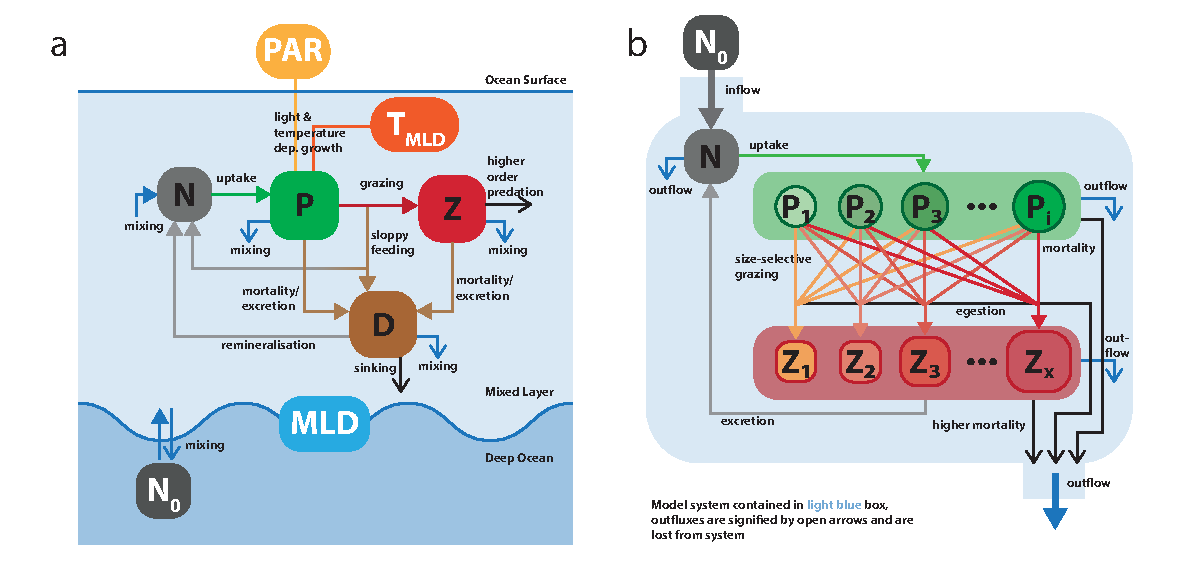
\includegraphics[width=15cm]{Figures/firstdraft_schematics/02__schematics_NPZDandChemostat.pdf}
\caption{TEXT}
\label{phydraschematics_1}
\end{figure*}

\subsubsection{Model Structure: Size-structured chemostat}

\subsubsection{Model Structure: Size-structured slab}
%%f
\begin{figure*}[t]
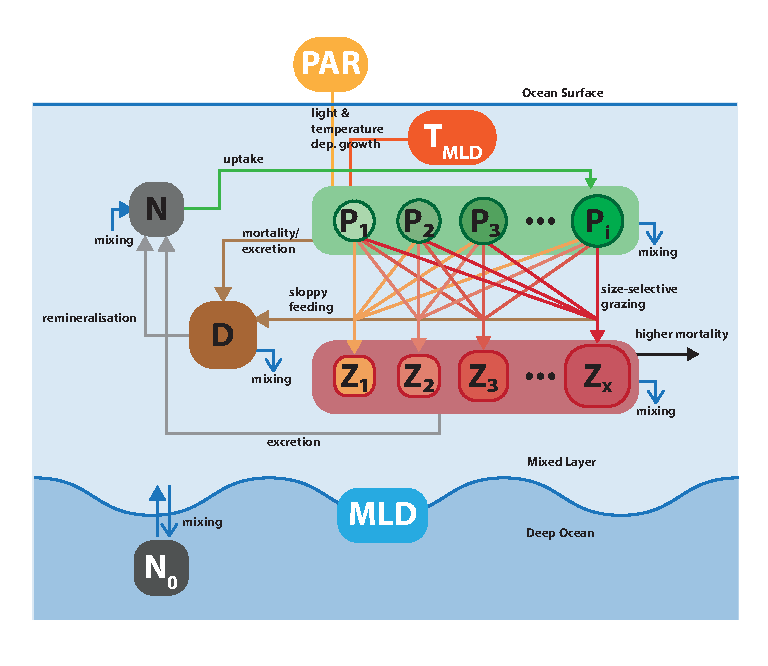
\includegraphics[width=10cm]{Figures/firstdraft_schematics/03__schematics_SizeStructSlab.pdf}
\caption{TEXT}
\label{phydraschematics_3}
\end{figure*}


% then move on to Results:
\subsection{Results}

\subsubsection{NPZD slab model}

%%f
\begin{figure}[t]
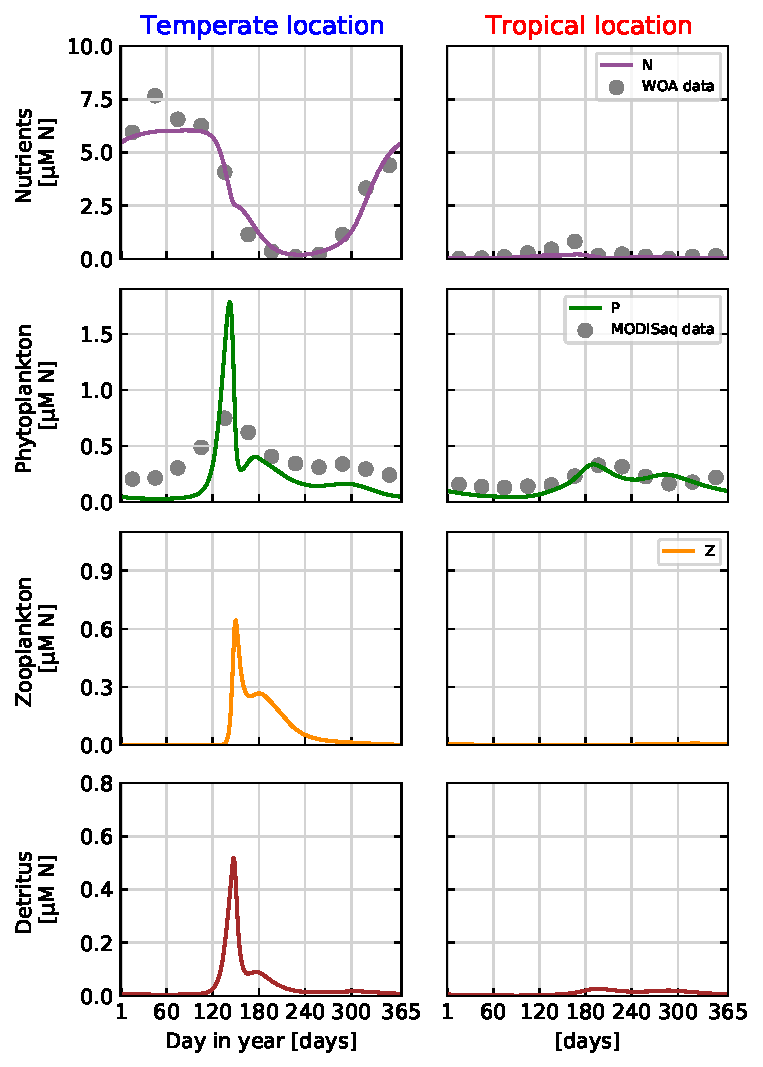
\includegraphics[width=6cm]{Figures/firstdraft_plots/02_NPZDslab.pdf}
\caption{TEXT}
\end{figure}

\subsubsection{Size-structured NP40Z40 chemostat model}
%%f
\begin{figure}[t]
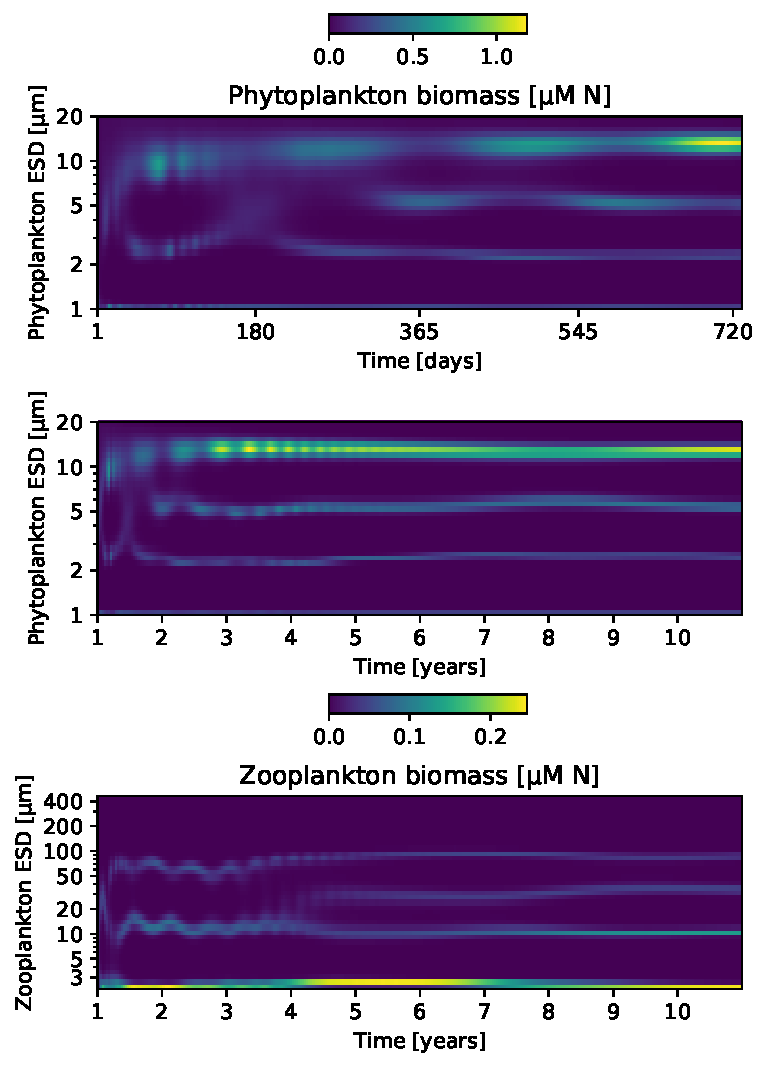
\includegraphics[width=6cm]{Figures/firstdraft_plots/03_chemostat.pdf}
\caption{TEXT}
\label{ASTroCAT_plot}
\end{figure}

\subsection{Size-structured NP20Z20D slab model}
%%f
\begin{figure*}[t]
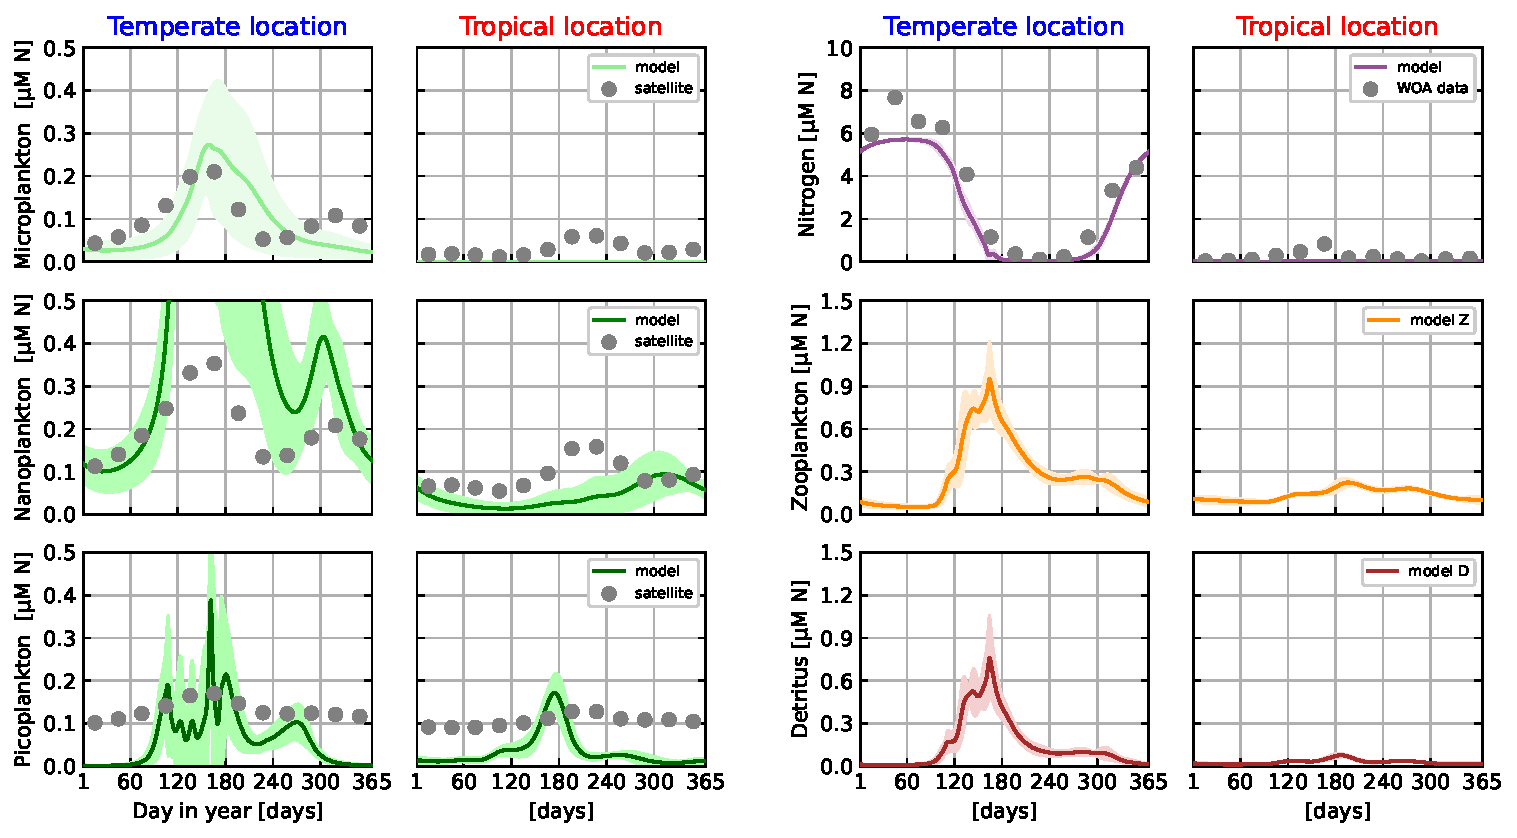
\includegraphics[width=12cm]{Figures/firstdraft_plots/04_sizestruct_slab.pdf}
\caption{TEXT}
\label{ASTroCAT_plot}
\end{figure*}


\end{document}